\begin{figure}
	\centering
	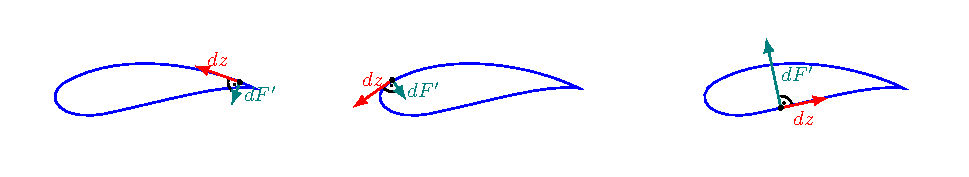
\includegraphics[width=\textwidth]{papers/joukowski/images/03_auftriebskraft/kontourintegral_fluegel.pdf}
	\caption{
		Die resultierende Kraft $F'$ ergibt sich durch das Aufsummieren aller kleiner Kraftanteilen $dF'$
		entlang der gesamten Kontur des Tragflügels.
		\label{joukowski:auftriebskraft:fig:kontourintegral-fluegel}}
\end{figure}
